%%%%%%%%%%%%%%%%%%%%%%%%%%%%%%%%%%%%%%%%%%%%%%%%%%%%%%%%%%%%%%%%%%%%%%%%%%%%%%%%%%%%%
\section{Future Directions: Multi-Messenger Dark Matter Search}\label{sec:future}
%%%%%%%%%%%%%%%%%%%%%%%%%%%%%%%%%%%%%%%%%%%%%%%%%%%%%%%%%%%%%%%%%%%%%%%%%%%%%%%%%%%%%

\begin{figure}[h]
    \centering{
        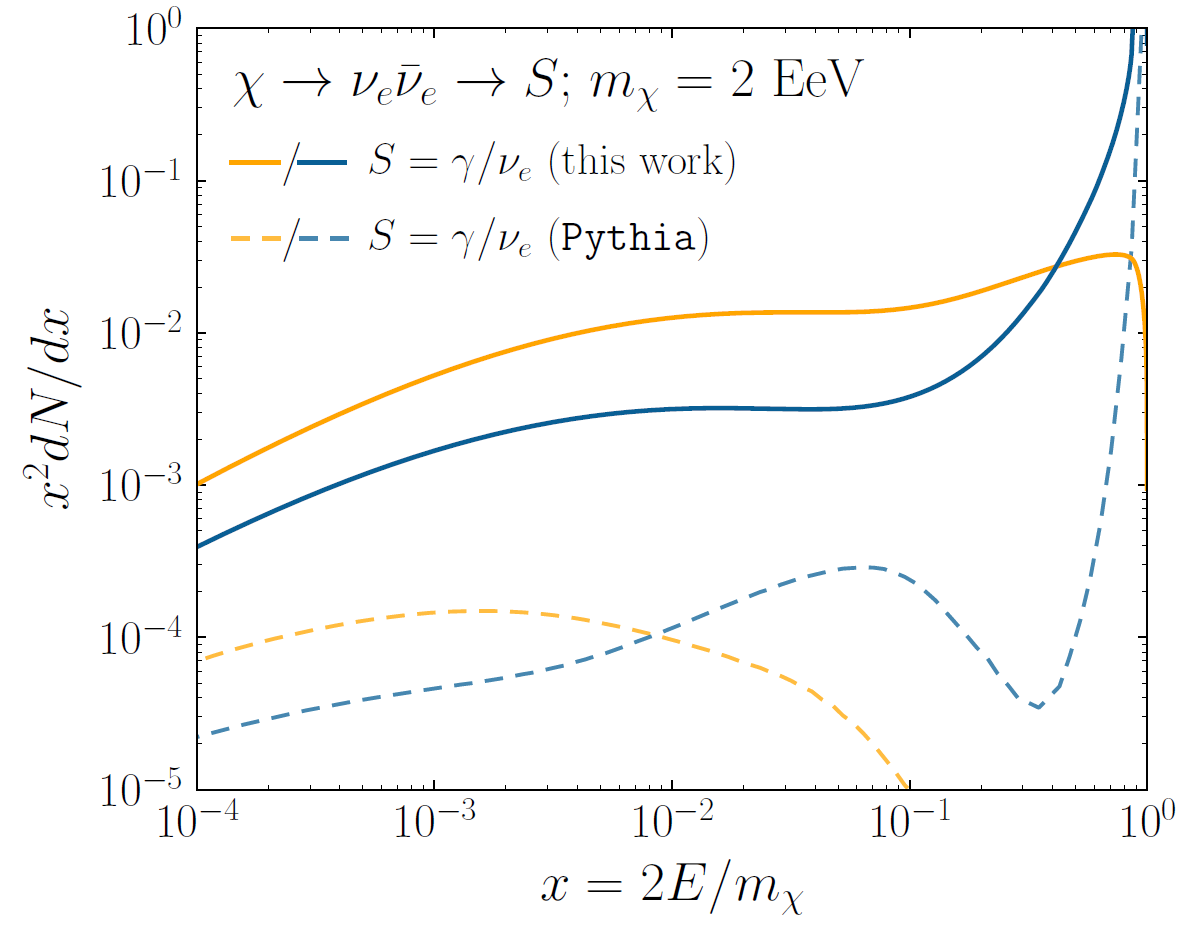
\includegraphics[scale=0.4]{figures/hdm_gamma_nu.png}
    }
    \caption{The $\nu_e$ and $\gamma$ spectrum at production from the decay of a 2 EeV DM particle to \parpar{\nu_e}. Solid lines are from the work of Nick Rodd et al. \cite{HDMSpectra}. Dashed lines are previous models produced by the [article physics framework \texttt{PYTHIA}. Notice that the flux for both $\nu_e$ and $\gamma$ are significantly larger than previously predicted, especially at low energies. Similar changes are seen in DM masses above the electroweak scale.}
    \label{fig:nu_and_gam}
\end{figure}

As I have shown previously in \Cref{sec:glory_duck} and \Cref{sec:multithread}, we can build a fast and robust analysis in HAWC that shares tools with the field.
Myself and the Glory Duck team have established a formalism for the purpose of combining common DM observations.
These combinations, \Cref{sec:glory_duck}, and accelerations,\Cref{sec:multithread}, laid the groundwork for faster DM searches without sacrificing on the scientific rigor.

\begin{figure}[t]
    \centering{
        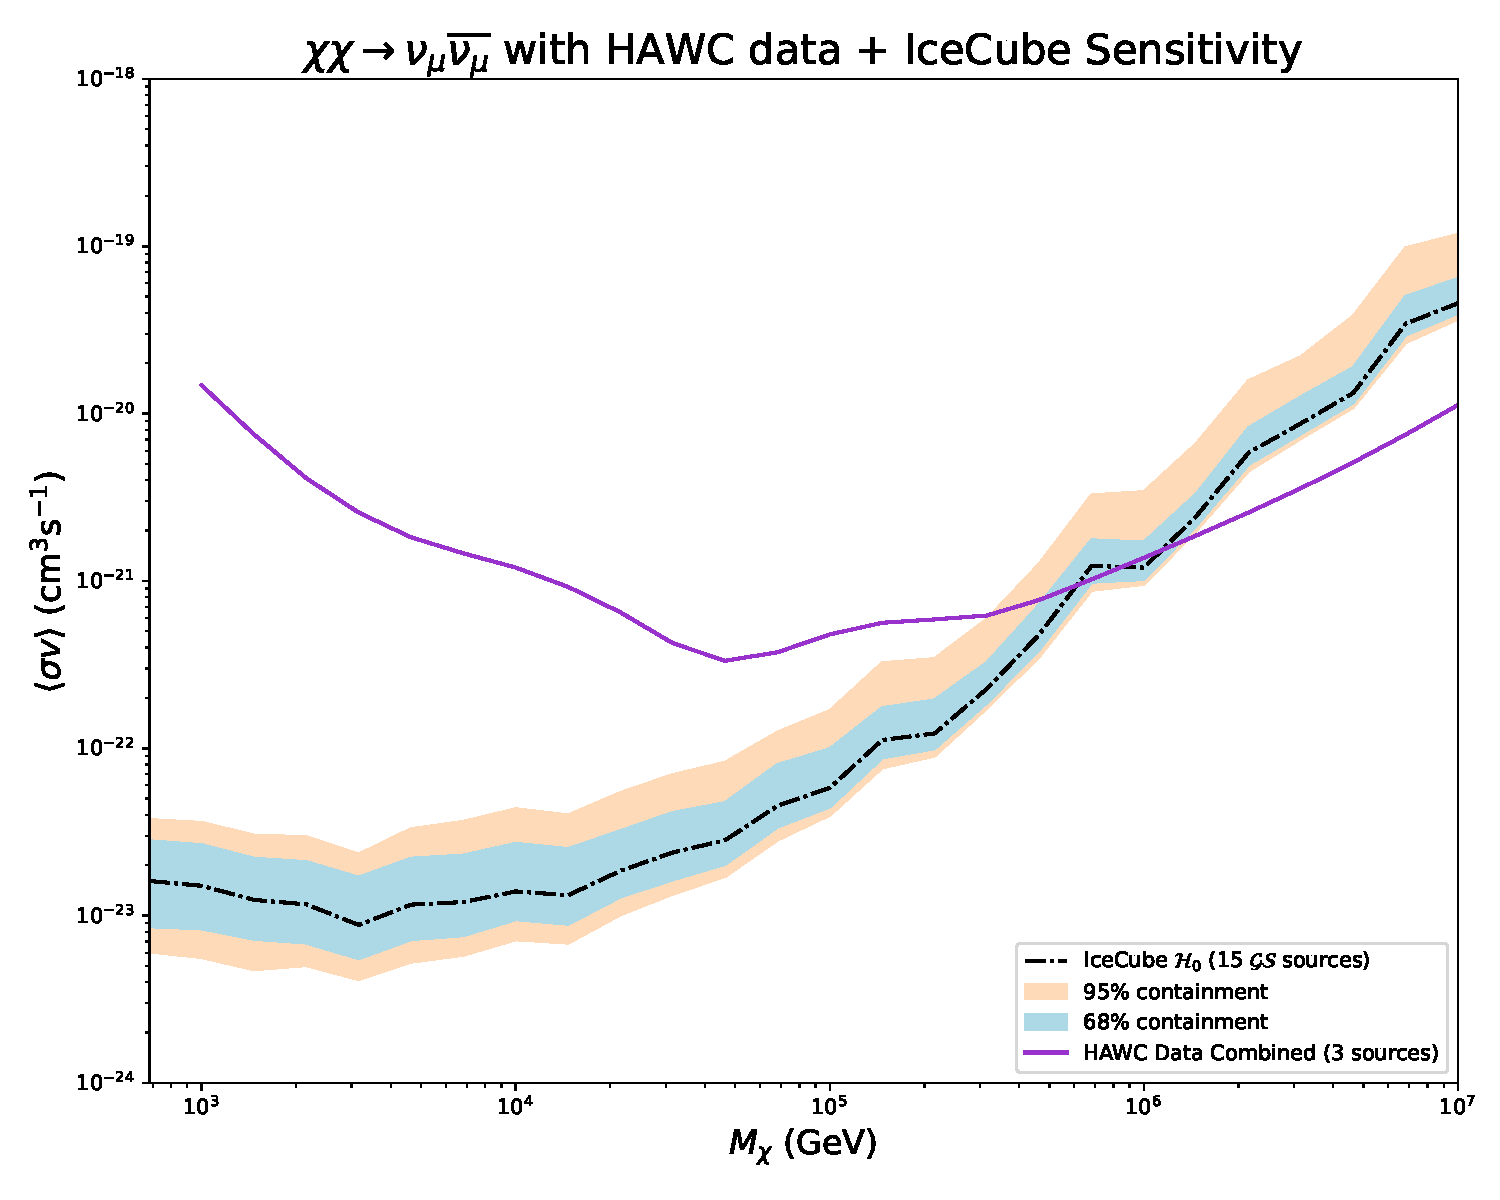
\includegraphics[scale=0.6]{figures/numunumu_hawcWic3_sens.pdf}
    }
    \caption{(purple line) HAWC 95\% confidence limit on \sv~using data from 3 sources: Coma Berenices, Segue 1, and Sextans. (Dashed black line) IceCube median 95\% confidence limit on \sv~over 300 background trials. Colored bands around $\mathcal{H}_0$ are the 68\% (light blue) and 95\% (peach) containment bands. The median IceCube value and HAWC data are most similar in the $m_\chi \approx 1$ PeV region.}
    \label{fig:nuDuck_sens}
\end{figure}

Within IceCube, I developed the first DM annihilation search towards dSphs in over a decade, \Cref{sec:ic3_dm}.
Moreover, this work was developed with the long-term goal: combining with gamma-ray data for a multi-messenger DM search.
There is already promising developments in DM phenomonalogy in this regard.
\Cref{fig:nu_and_gam} is the headline figure from \texttt{HDMSpectra} \cite{HDMSpectra} for a DM decay ($\chi \rightarrow$\parpar{\nu_e}) spectrum in $\nu_e$~ and $\gamma$.
What is intriguing from this publication is that although photons more readily interact with our detector than neutrinos, the expected photon spectrum is soft enough to be difficult to discern from the background.
Whereas, I showed that IceCube has exceptional sensitivity for hard neutrino spectra, see \cref{fig:icDM_stact_numu_TS,fig:icDM_sensitivity_2of2}.
Additionally, the Earth was going to play a role in reducing IceCube's neutrino sensitivity, see \cref{fig:icDM_dec_study} and \cite{IC3:Earth_Attenuation}.
These known behaviours clued us in on a potentially powerful partnership with HAWC and IceCube.

Here I show some of the preliminary work done to combine HAWC and IceCube data for a multi-messenger DM search.
My IceCube analysis, \Cref{sec:ic3_dm}, through background simulation, showed that our variables behave mostly like normal variables distributed as a $\chi^2$ distribution with 1 degree of freedom.
For IceCube we adopt the statistical framework for setting confidence limits first made by Fermi-LAT \cite{FermiLAT:dm1}, and later Glory Duck, \cref{sec:gd_joint_llh}.
I adopt, in IceCube, the 95\% confidence limit standard defined in \cref{eq:hawc_cl95} with a likelihood combination from \cref{eq:gdJointLLH}.
This differs from the 90\% confidence limit considered standard within IceCube and used for \Cref{sec:ic3_dm}.
This statistical definition is standard for HAWC and requires no additional changes than what was presented in \Cref{sec:multithread}.

I calculated sensitivities for IceCube on 300 background trials and present the median, 68 and 95 percentile containment on the confidence limit with IceCube NST.
The source and model selection for IceCube is identical to \cref{sec:ic3_study_selection}.
I also calculate the confidence limit for HAWC using the methods and dataset from \cref{sec:mtd_srcs_y_chan} but the source models (\GS) from \cref{sec:gd_srcs_y_chan}.
HAWC did not have an unblinding process, yet IceCube does.
Therefore, IceCube data is not represented.
\Cref{fig:nuDuck_sens} features IceCube's sensitivity suerimposed on HAWC's 95\% confidence limit on DM annihilation: $\chi\chi \rightarrow$ \parpar{\nu_\mu}.
We can see that IceCube's sensitivity is complimented well by HAWC's confidence limit in the DM mass region above and around 1 PeV.

I also do a mock combination between HAWC and IceCube.
This mock run was made for the purpose of building the neutrino + gamma data pipeline for DM searches.
\Cref{fig:nuDuck_mockdata} shows a combined limit between HAWC data and an IceCube simulated background trial treated as data.
In this exersize we see that we indeed have a powerful combination in the 1 PeV DM mass region.
We see an improvement to the combined limit to as far down as 100 TeV in DM mass.
Furthermore, the improvement to this limit stay across two decades in DM mass.
This preliminary work is evidence of the strength in multi-messenger DM searches and motivates such a study between these instruments.

\begin{figure}
    \centering{
        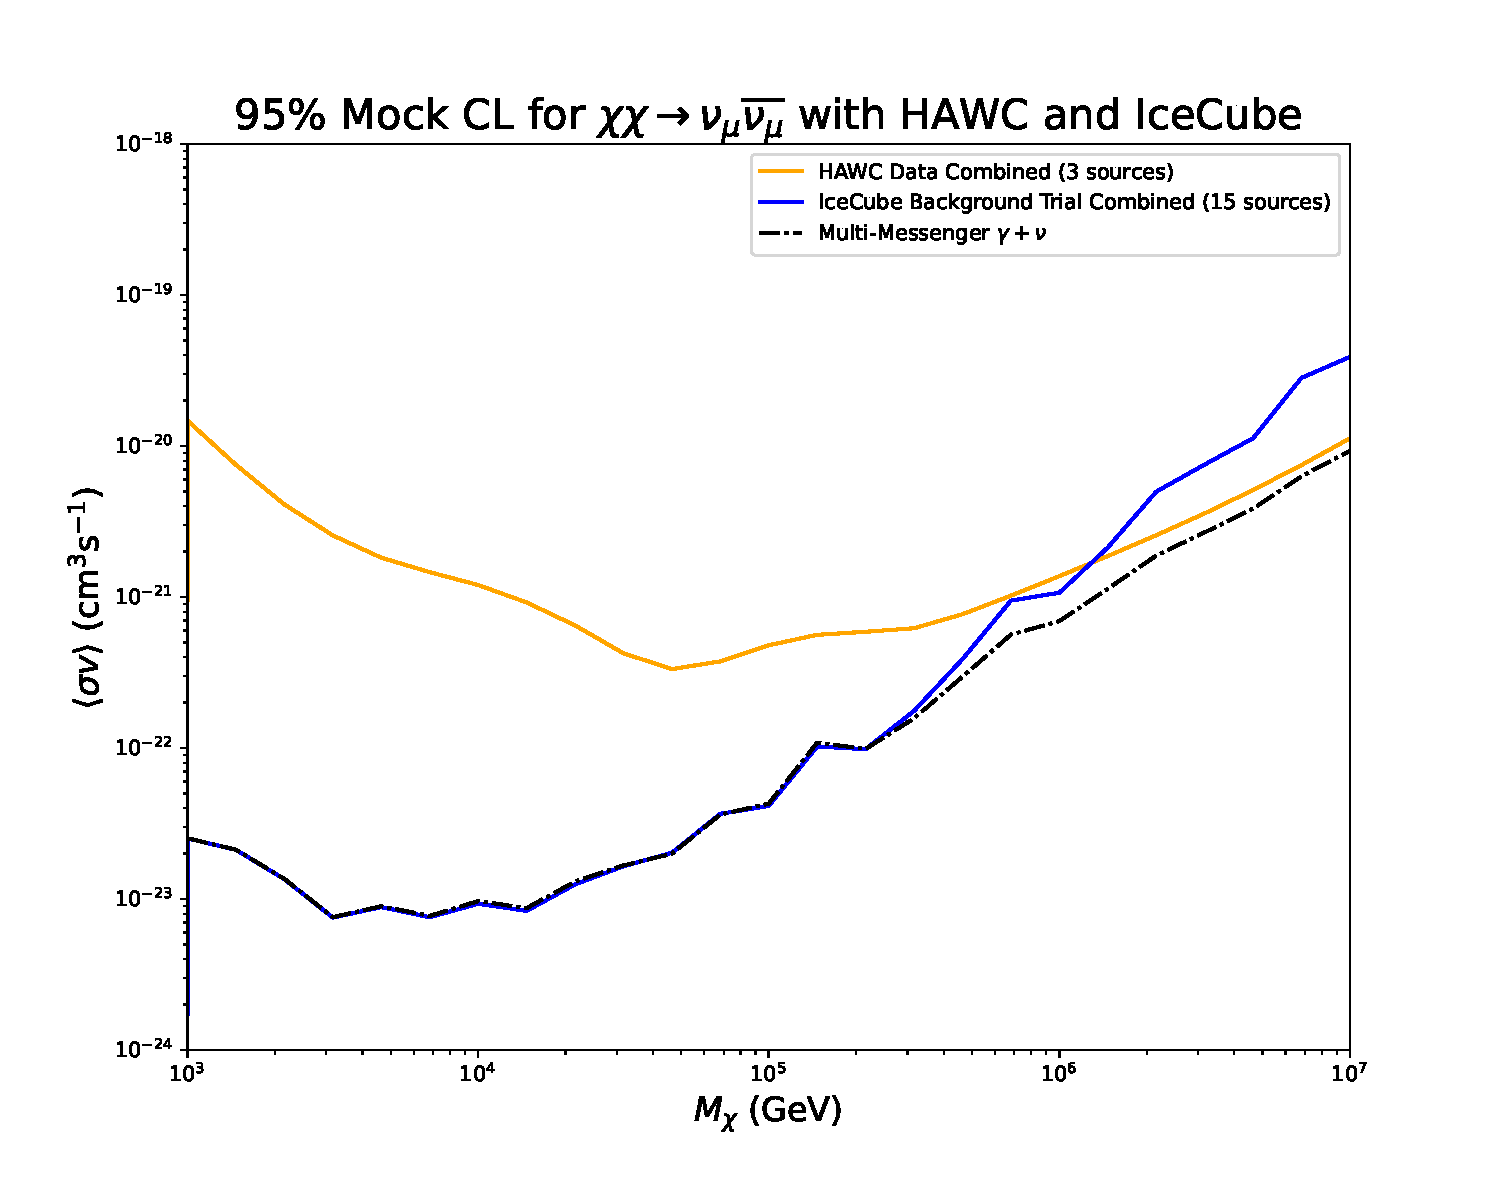
\includegraphics[scale=0.6]{figures/numunumu_mock_data.pdf}
    }
    \caption{(orange solid line) HAWC 95\% confidence limit on \sv~using data from 3 sources: Coma Berenices, Segue 1, and Sextans. (blue solid line) IceCube 95\% confidence limit on \sv~from one simulated background trial. (dashed black line) Combined 95\% confidence limit on \sv~with HAWC data and IceCube background trial. Combined limit is stronger than either IceCube and HAWC in the region $m_\chi > 200$ TeV. }
    \label{fig:nuDuck_mockdata}
\end{figure}

%%%%%%%%%%%%%%%%%%%%%%%%%%%%%%%%%%%%%%%%%%%%%%%%%%%%%%%%%%%%%%%%%%%%%%%%%%%%%%%%%%%%%
\section{Conclusions}\label{sec:conclusions}
%%%%%%%%%%%%%%%%%%%%%%%%%%%%%%%%%%%%%%%%%%%%%%%%%%%%%%%%%%%%%%%%%%%%%%%%%%%%%%%%%%%%%

This dissertation, "Leveraging Multi-Messenger Astrophysics for Dark Matter Searches," advances our quest to understand dark matter. We used gamma-ray and neutrino observatories alongside advanced computational techniques. Our goal was to enhance the search for dark matter within the universe.

The Glory Duck project was a key part of this work. It involved a multi-instrument analysis using gamma-ray telescopes. These included Fermi-LAT, H.E.S.S., MAGIC, VERITAS, and HAWC. They focused on 20 dwarf spheroidal galaxies (dSphs). The aim was to detect dark matter annihilation signals. Although we found no significant deviations from the null hypothesis, we greatly improved search sensitivity. We set stringent upper limits on the annihilation cross-section for dark matter candidates. This effort represents a major advance, offering the most comprehensive constraints for WIMP dark matter search to date.

Our exploration of multithreading techniques in HAWC analyses showed the benefits of computational methods. By accelerating analysis time, we enhanced the efficiency of dark matter searches. This approach has set the stage for more ambitious studies. It highlights the importance of computational innovation in addressing astrophysical challenges.

Furthermore, our work with IceCube's North Sky Track Data has broken new ground. It aimed at detecting heavy dark matter annihilation. We used parallel programming and spline fitting to improve IceCube's sensitivity. This analysis is a step towards probing dark matter annihilation up to the PeV scale. It demonstrates a significant sensitivity improvement compared to previous efforts. The groundwork laid here is a strong foundation for future discoveries.

This dissertation highlights the potential of multi-messenger astrophysics and computational innovation in dark matter searches. Each analysis has contributed to our understanding and capabilities. Together, they showcase a progressive approach to astrophysical research. By integrating observations and using the latest computational techniques, we have expanded our capabilities. We have also charted a path for future dark matter searches.

Looking back, it's clear that our journey through the dark universe is far from complete. The methods developed and findings reported here significantly contribute to the astrophysical community. They set the stage for future multi-messenger observations and analyses. In this pursuit, the challenges we face and the questions we seek to answer drive us forward. They fuel the continuous evolution of our search for dark matter.
